The tests have been conducted on a linux machine, kernel SMP 3.13.11, equipped with a Quad core CPU Intel Core i7-4700MQ CPU @ 2.40GHz (Turbo-Boost up to 3.4GHz) with support for HyperThreading technology which enables each core to handle efficiently up to two threads.\\
The test consists of encrypting a file, decrypting it, and comparing the decrypted one with the original to check functional correctness. The files used for the tests range in dimension from few hundreds of KB to 4GB, but there is no limit on the size of the input file apart from the kernel limit and the upper bound imposed by the 64 bits variable for addresses.\\
Every file have been tested with 1, 2, 4 and 8 threads (the maximum parallelism allowed by the hardware).\\
The results are the following:

\begin{figure}[H]
\centering
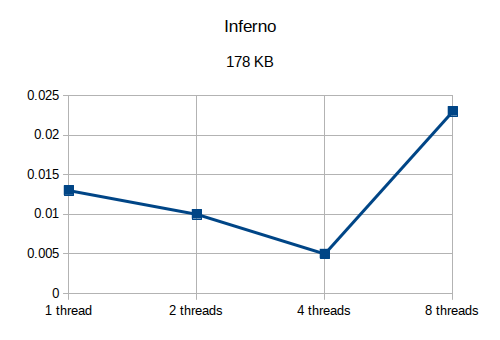
\includegraphics[scale = 0.8]{./Pictures/Inferno} % x compreso tra 0 e 1
\caption{Inferno}
\label{fig:Inferno}
\end{figure}

\begin{figure}[H]
\centering
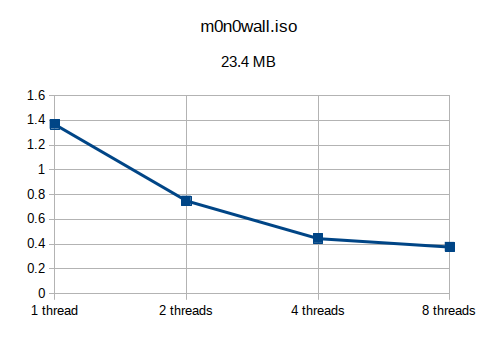
\includegraphics[scale = 0.8]{./Pictures/m0n0wall} % x compreso tra 0 e 1
\caption{m0n0wall}
\label{fig:m0n0wall}
\end{figure}

\begin{figure}[H]
\centering
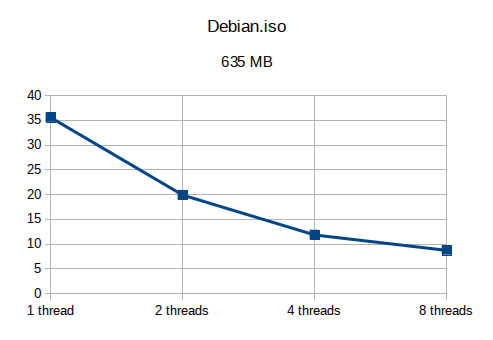
\includegraphics[scale = 0.8]{./Pictures/Debian} % x compreso tra 0 e 1
\caption{Debian}
\label{fig:Debian}
\end{figure}

\begin{figure}[H]
\centering
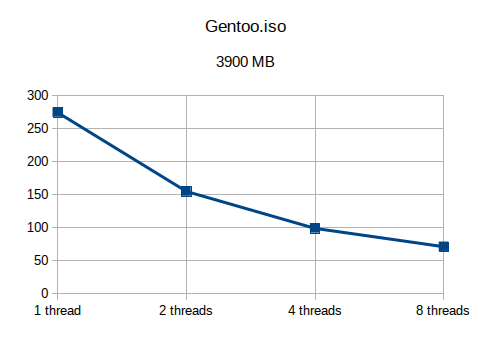
\includegraphics[scale = 0.8]{./Pictures/Gentoo} % x compreso tra 0 e 1
\caption{Gentoo}
\label{fig:Gentoo}
\end{figure}

As we can see, apart for an anomaly in the first test due to the fact that the file was really too small for such an high number of threads, the algorithm scales very well and can handle well also very big files.\\
Doubling the number of threads lead to a speedup which range from 1.4 to 1.82.

\subparagraph{Script}
The test script is the following:

\begin{scripting}
\begin{verbatim}
#!/bin/sh
#set -xv

# WARNING: diff fail in case of final new line in input file

BUILD_DIR=./build
TEST_DIR=./test

TEST_FILE=test_input
KEY="0000000000000000"
MAX_THREADS=8
DEBUG=0

EXECUTABLE=$BUILD_DIR/blowfish-multithread
INPUT=$TEST_DIR/$TEST_FILE
ENC_OUTPUT=$TEST_DIR/enc_output
DEC_OUTPUT=$TEST_DIR/dec_output

ENC_LOGFILE=$TEST_DIR/enc.log
DEC_LOGFILE=$TEST_DIR/dec.log



if [ "$DEBUG" == "1" ]; then
	EXECUTABLE="gdb --args $EXECUTABLE"
fi


echo "clean"
if [ -a "$ENC_OUTPUT" ]; then
	rm "$ENC_OUTPUT"
fi

if [ -a "$DEC_OUTPUT" ]; then
	rm "$DEC_OUTPUT"
fi

echo "encrypt"
$EXECUTABLE "e" "$INPUT" "$KEY" "$ENC_OUTPUT" "$MAX_THREADS" #> "$ENC_LOGFILE"
echo ""

echo "decrypt"
$EXECUTABLE "d" "$ENC_OUTPUT" "$KEY" "$DEC_OUTPUT" "$MAX_THREADS" #> "$DEC_LOGFILE"
echo ""

echo "comparing"
if diff -B -b -E -Z "$INPUT" "$DEC_OUTPUT" >/dev/null ; then
	echo -e "\e[00;32mOK\e[00m"
else
	echo -e "\e[00;31mDifferent\e[00m"
fi
\end{verbatim}
\end{scripting}